\section*{Zielsetzung}
\label{sec:Zielsetzung}
In diesem Versuch sollen verschiedene Phänomene, die bei gekoppelten Pendeln auftreten,
untersucht werden. Im Fokus steht dabei die Schwebung.

\section{Theorie}
\label{sec:Theorie}
Wichtige Kenngrößen beim Pendel sind die Fadenlänge $l$ und Masse $m$. Wird das Pendel
ausgelenkt, so sorgt die Gewichtskraft mit ihrer tangentialen Komponente für ein
Drehmoment $M = D_p \cdot \phi$, wobei $\phi$ der Auslenkwinkel und $D_p$ die
Winkelrichtgröße des Pendels sind. Bei kleinen Winkeln ($\phi \leq 10^\circ$) 
folgt aus der linearen Taylorentwicklung die Näherung $\sin(\phi) \approx \phi$.
Damit lässt sich die Bewegungsgleichung des Pendels
\begin{equation}
	J \cdot \ddot \phi + D_p \phi = 0
	\label{eqn:dgl-harm-osz}
\end{equation}
aufstellen, mit dem Trägheitsmoment $J$. Diese DGL wird durch eine harmonische Schwingung
mit der Frequenz
\begin{equation}
	\omega = \sqrt{\frac{D_p}{J}} = \sqrt{\frac{g}{l}}.
\end{equation}
Bemerkenswert ist dabei die Tatsache, dass $\omega$ komplett unabhängig von Pendelmasse
und dem Auslenkwinkel $\phi$ ist.
\\
In diesem Versuch sollen gezielt gekoppelte Pendel betrachtet werden; die Kopplung wird hier durch
eine Feder realisiert. Diese sorgt für ein zusätzliches Drehmoment 
$M_1 = D_F (\phi_2 - \phi_1)$ aufs erste bzw. $M_2 = D_F (\phi_1 - \phi_2)$ auf das zweite
Pendel. Aus \autoref{eqn:dgl-harm-osz} folgt ein System gekoppelter Differentialgleichung 
\begin{align}
	J \ddot \phi_1 + D \phi_1 &= D_F (\phi_2 - \phi_1), \\
	J \ddot \phi_2 + D \phi_2 &= D_F (\phi_1 - \phi_2).
\end{align}
Durch eine Variablensubstitution können diese entkoppelt werden und als zwei unabhängige,
harmonische Schwingungen dargestellt werden. Die Frequenzen dieser zwei Schwingungen
werden mit $\omega_1$ und $\omega_2$ bezeichnet, die Auslenkwinkel der Pendel $\alpha_i$.
Abhängig von den Anfangsbedingungen $\alpha(t = 0)$ und $\dot \alpha(t = 0)$ können dabei
drei Schwingungsarten auftreten, welche in \autoref{fig:3schwingungen} dargestellt sind.
\begin{itemize}
	\item \textbf{Gleichsinnige Schwingung:} $\alpha_1 = \alpha_2$ \\
		Im Fall gleicher Auslenkung übt die Feder keine Kraft aus. Die
		Schwingungsfrequenz ist daher unverändert $\omega_+ = \sqrt{\frac{g}{l}}$.
		Die Schwingungsdauer folgt dann mit
		\begin{equation}
			T_+ = 2\pi \sqrt\frac{l}{g}.
			\label{eqn:T_+}
		\end{equation}
	\item \textbf{Gegensinnige Schwingung:} $\alpha_1 = -\alpha_2$ \\
		Der zweite Sonderfall ist der Fall entgegengesetzter Schwingung. Da die
		Feder jetzt die rücktreibende Kraft unterstützt, liegt hier eine höhere
		Schwingungsfrequenz 
		\[
			\omega_- = \sqrt{\frac gl + \frac{2K}{l}}
		\]
		vor, mit der Kopplungskonstante $K$, welcher von der Feder abhängt. 
		Damit folgt die Schwingungsdauer
		\begin{equation}
			T_- = \frac{2\pi}{\omega_-} = 2\pi \sqrt{\frac{l}{g+2K}}. \label{eqn:t-}
		\end{equation}
	\item \textbf{Gekoppelte Schwingung:} $\alpha_1 = 0, \alpha_2 \neq 0$ \\
		Zuletzt wird der Fall der gekoppelten Schwingung betrachtet. Hier wird ein
		Pendel in Ruhelage gelassen und das zweite um $\alpha_2$ ausgelenkt. Die
		Energie, welche anfangs in nur einem Pendel vorliegt, wird langsam auf das
		Zweite übertragen und wandert dann periodisch zwischen beiden hin und her.
		Dieses Phänomen wird als \textit{Schwebung} bezeichnet und hat
		Periodendauer und Frequenz
		\begin{equation}
			\label{eqn:ts}
			T_S = \frac{T_+ \cdot T_-}{T_+ - T_-}
			\quad
			\text{und}
			\quad
			\omega_S = \omega_+ - \omega_-.
		\end{equation}
		Damit kann dann auch die Kopplungskonstante 
		\begin{equation}
			K = \frac{\omega_-^2 - \omega_+^2}{\omega_-^2 + \omega_+^2}
			=\frac{T_+^2 - T_-^2}{T_+^2 + T_-^2}
			\label{eqn:kopplungskonstante}
		\end{equation}
		bestimmt werden.
\end{itemize}
\begin{figure}[H]
	\centering
	\begin{subfigure}[b]{0.3\textwidth}
		\centering
		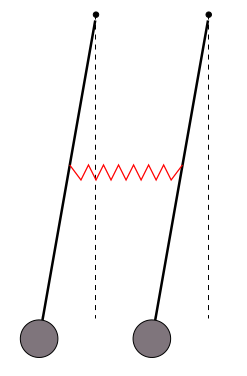
\includegraphics[width=\textwidth]{images/gleichsinnig.png}
		\caption{Gleichsinnige Schwingung.}
		\label{fig:gleichsinnig}
	\end{subfigure}
	\hfill
	\begin{subfigure}[b]{0.3\textwidth}
		\centering
		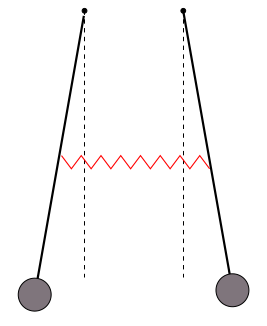
\includegraphics[width=\textwidth]{images/gegensinnig.png}
		\caption{Gegensinnige Schwingung.}
		\label{fig:gegensinnig}
	\end{subfigure}
	\hfill
	\begin{subfigure}[b]{0.3\textwidth}
		\centering
		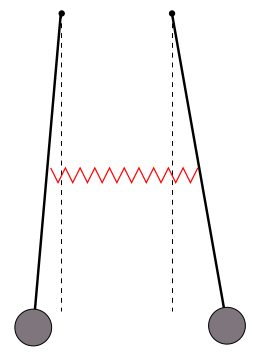
\includegraphics[width=\textwidth]{images/gekoppelte.png}
		\caption{Gekoppelte Schwingung.}
		\label{fig:gekoppelt}
	\end{subfigure}
	\caption{Die drei charakteristischen Schwingsarten grafisch dargestellt.
	\cite{sample}}
	\label{fig:3schwingungen}
\end{figure}

